\section{From the linear seed to a nonlinear height}
\label{sec:solving-the-equation}
\label{sec:exact-return-height}

We can now see why the unknowns were chosen as they were. The height
solves the curvature equation. One compact metric parameter removes
its second-mode obstruction. One radial control per negative component
adjusts the mean travel angle. Finally the odd boundary charts adjust
the nonconstant return maps. The last two tasks are separated by taking
the angular mean. Their feedback through the height contains the small
amplitude $q$, which makes the coupled linear problem invertible.

\subsection{The residual and its four unknowns}

Use the state \eqref{eq:rewrite-state}, with $q\in\R$ a parameter.
Set
\begin{equation}\label{eq:readable-joint-residual}
 \mathcal R(\mathbf x,q)=(\mathcal A,\mathfrak e),
 \qquad \mathcal A=\mathcal F_q(w,u),
 \qquad \mathfrak e=\mathfrak e(qu,\kappa,h_L).
\end{equation}
The tangent and residual spaces are
\[
 \mathfrak X=(\mathcal X_\beta\cap\ker\ell_*)\times\R
       \times\mathcal K_\beta\times\mathcal Z_{\beta,\mathrm{odd}},
 \qquad
 \mathfrak Y=\mathcal Y_\beta\times\mathcal Z_{\beta,\mathrm{even}}.
\]
The second residual space includes its angular means. The scalar
space uses the integral compatibility from the connection form.
The normalized scalar equation is smooth through $q=0$ by
\eqref{eq:normalized-integral}. The coefficient and flow calculus of
Section~\ref{sec:fixed-geometry} makes $\mathcal R$ smooth tame on
one open neighborhood $\mathfrak n_{b_0}<\epsilon_0$.
At
\[
 q=0,\qquad \mathbf x_0=(\Phi_*,0,0,\id)
\]
it is zero: $\mathscr L_{w_*}\Phi_*=0$ and the reference return maps
are the prescribed rotations.

Write the differentiated circle rows as
\begin{equation}\label{eq:joint-circle-linear-rows}
 C_{\mathbf x}^{\circ}=D_Z\mathfrak e,\quad
 R_{\mathbf x}^{\circ}=\av{C_{\mathbf x}^{\circ}},\quad
 \mathcal D_{\mathbf x}=D_\kappa\mathfrak e,\quad
 J_{\mathbf x}=\av{\mathcal D_{\mathbf x}}.
\end{equation}
The map on component $m$ depends on its height jets, its chart and
$\kappa_m$. It does not depend on $\nu$ or the endpoint scalar,
whose positive jets are supported in positive components.
Thus $J_{\mathbf x}$ is diagonal. At a radial state
$\mathfrak e=T(w)-T(w_*)$, so the normalization of the controls gives
$J_0=I$. On one small low-order neighborhood its entries are uniformly
separated from zero and its inverse is smooth tame.

The reference mean derivative annihilates nonzero height frequencies
and odd chart directions. For a radial increment $Z$ it is
\begin{equation}\label{eq:rewrite-reference-circle-row}
 (R_0^\circ Z)_m
 =-\int_{I_m}v_0\frac{1+w_*^2}{w_*}Z_r\,dr.
\end{equation}
To verify this, at a radial state the speed is
$v_0w_*\sqrt D/(w_*+Z_r)$, with
$D=1-2w_*Z_r-Z_r^2$. Its logarithmic variation is
$-(1+w_*^2)Z_r/w_*$. Angular translation invariance gives the
nonzero-mode assertion. In particular $R_0^\circ\Phi_*=0$.

With $K_{\mathbf x}=D_\kappa\mathcal A$ and
$k_{\mathbf x}=D_\nu\mathcal A$, the corrected linear equations are
\begin{equation}\label{eq:corrected-coupled-linear-system}
 \begin{split}
 \widehat L_{\mathbf x}\eta+k_{\mathbf x}\mu+K_{\mathbf x}\xi&=f,
                    \qquad \ell_*\eta=0,\\
 qC_{\mathbf x}^{\circ}\eta+\mathcal D_{\mathbf x}\xi
                            +\mathcal M_Tv&=g.
 \end{split}
\end{equation}
The actual chart variation is $v\circ h_L$. The equation differs
from the true derivative only by the two residual terms already
identified and the chart error in
\eqref{eq:full-height-chart-derivative}.

\begin{figure}[htbp]
\centering
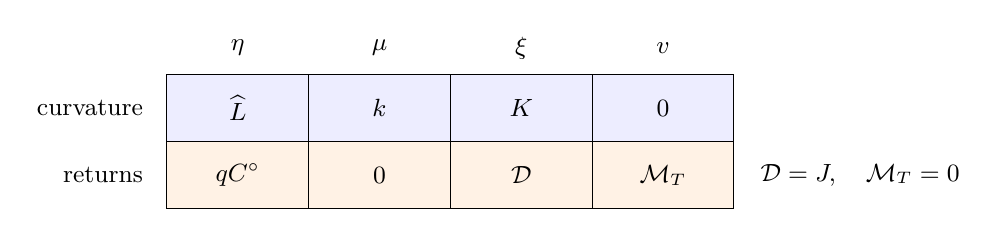
\begin{tikzpicture}[x=1.8cm,y=.85cm,font=\small]
\fill[blue!7] (0,1) rectangle (4,2);
\fill[orange!10] (0,0) rectangle (4,1);
\draw (0,0) rectangle (4,2);
\draw (0,1)--(4,1);
\foreach \x in {1,2,3} {\draw (\x,0)--(\x,2);}
\node at (.5,2.4) {$\eta$}; \node at (1.5,2.4) {$\mu$};
\node at (2.5,2.4) {$\xi$}; \node at (3.5,2.4) {$v$};
\node at (.5,1.5) {$\widehat L$}; \node at (1.5,1.5) {$k$};
\node at (2.5,1.5) {$K$}; \node at (3.5,1.5) {$0$};
\node at (.5,.5) {$qC^\circ$}; \node at (1.5,.5) {$0$};
\node at (2.5,.5) {$\mathcal D$}; \node at (3.5,.5) {$\mathcal M_T$};
\node[anchor=east] at (-.1,1.5) {curvature};
\node[anchor=east] at (-.1,.5) {returns};
\node[anchor=west] at (4.12,.5) {$\av{\mathcal D}=J,\quad\av{\mathcal M_T}=0$};
\end{tikzpicture}
\caption{The corrected derivative and the roles of its four columns.
Taking the mean of the second row removes the chart column. Feedback
from that row to the height is multiplied by $q$.}
\label{fig:coupled-columns}
\end{figure}

\subsection{The control contribution gains all component weights}

Let $G_{\mathbf x}$ be the scalar inverse of
Proposition~\ref{prop:rewrite-volume-inverse} and set
$U_{\mathbf x}=G_{\mathbf x}K_{\mathbf x}$.
The useful base space for control increments is
\[
 B_\beta=\left\{\xi:\sum_mH_m^{-2\beta}|\xi_m|^2<\infty\right\}.
\]
For every $s$, with a fixed loss $d_*$,
\begin{equation}\label{eq:weak-control-smoothing}
 \|K_{\mathbf x}\xi\|_{\mathcal Y_\beta,s}
 +\|U_{\mathbf x}\xi\|_{\mathcal X_\beta,s}\!+|(U_{\mathbf x}\xi)_{\mu}|
 \le C_s(1+\mathfrak n_{s+d_*})\|\xi\|_{B_\beta}.
\end{equation}
In the middle term the norm denotes the height component of $U\xi$.

Here is the reason for this strong smoothing in the component index.
Differentiate the removable formula for $\mathcal F_q$ with respect
to a control. Every term contains that control increment and a
positive height jet: the curvature expression is unchanged by adding
a constant to the height. This remains true at $q=0$, where the
derivative is that of $\mathscr L_wu$. On component $m$ write
$\xi_m=H_m^\beta b_m$. The height jet contributes another
$H_m^\beta$. After dividing by the source weight there remains a
factor $H_m^\beta$, which absorbs every fixed power of $M_m$ and
every complete coefficient product. The endpoint scalar has no
height jet on these control supports. The local product bound puts
one state factor at high order, and summation of $|b_m|^2$ gives the
estimate for $K$. Composing with $G$ adds only its fixed loss.

\subsection{Solving the coupled equations}

Put $g_0=\av g$. Solving the first row of
\eqref{eq:corrected-coupled-linear-system} gives
$y=(\eta,\mu)=Gf-U\xi$. Taking the mean of the second then gives
\[
 (I-qJ^{-1}R^\circ U)\xi
              =J^{-1}(g_0-qR^\circ Gf).
\]
The rows act on the height component of $G$ and $U$.
By \eqref{eq:weak-control-smoothing}, $R^\circ U$ is bounded on
the \emph{same} $B_\beta$, with a constant controlled by finitely
many state norms. Choose the low neighborhood to control those norms,
then choose $|q|$ so that
$\|qJ^{-1}R^\circ U\|_{B_\beta\to B_\beta}<1/2$.
The solution is therefore
\begin{equation}\label{eq:joint-height-circle-inverse}
 \begin{split}
 \xi&=(I-qJ^{-1}R^\circ U)^{-1}J^{-1}(g_0-qR^\circ Gf),\\
 (\eta,\mu)&=Gf-U\xi,\\
 v&=\mathcal M_T^{-1}(g-qC^\circ\eta-\mathcal D\xi).
 \end{split}
\end{equation}
The last argument has zero mean by the first equation, so the inverse
in \eqref{eq:rewrite-circle-inverse} applies.

Higher control norms come from the already solved identity
\[
 \xi=J^{-1}(g_0-qR^\circ Gf)+qJ^{-1}R^\circ U\xi.
\]
The final term has every higher norm using only
$\|\xi\|_{B_\beta}$ and one high state norm, by the smoothing
estimate. The first has the requisite source norms with fixed loss.
Consequently the same solution lies in all control spaces, with a
tame bound. Substitution gives the height and chart estimates.
The resolvent identity proves base continuity; this identity and its
higher estimates prove continuity in every order. Hamilton's
inverse-family theorem applies to the control inverse, making all
three formulas smooth tame. Thus
\[
 V(\mathbf x,q)(f,g)=(\eta,\mu,\xi,v\circ h_L)
\]
is a smooth tame map, linear in the residual pair.

\subsection{The exact quadratic-error identity}

We invoke Hamilton's implicit theorem with quadratic error
\cite[III, Theorem~3.3.1, pp.~211--212]{Hamilton1982}.
In the notation here its hypothesis is a smooth tame $\mathcal R$
on an open subset of tame spaces, together with a linear smooth tame
$V$ and a bilinear smooth tame $\mathcal Q$ such that
\begin{equation}\label{eq:rewrite-hamilton-hypothesis}
 D_{\mathbf x}\mathcal R\,V y
                  =y+\mathcal Q(\mathbf x,q)[\mathcal R,y].
\end{equation}
At an initial zero this gives a local smooth tame solution branch in
the parameter. We check the identity with two \emph{independent}
residual arguments; an informal quadratic bound would not suffice.

For the increments in \eqref{eq:joint-height-circle-inverse}, the
actual derivative is
\begin{equation}\label{eq:joint-height-circle-quadratic-error}
 D_{\mathbf x}\mathcal R(\eta,\mu,\xi,v\circ h_L)
 =\bigl(f+q\partial_\theta(B\mathcal A\eta_\theta)
              +\mathscr E_{\mathbf x}(\mathfrak e)\eta,
        \ g+\mathcal Q_h(\mathfrak e,v)\bigr).
\end{equation}
For $r=(r_1,r_2)$ and $y=(f,g)$ define
\[
 \mathcal Q(\mathbf x,q)[r,y]
 =\bigl(q\partial_\theta(Br_1\eta_\theta)
                   +\mathscr E_{\mathbf x}(r_2)\eta,
              \mathcal Q_h(r_2,v)\bigr).
\]
In $\mathcal Q_h$ keep the actual state paths in
\eqref{eq:full-height-chart-derivative}, replacing only its explicit
$\mathfrak e,\mathfrak e'$ factors by $r_2,r_2'$.
The same convention was built into $\mathscr E$.
The increments are linear in $y$, so this formula is bilinear in
$(r,y)$ and gives \eqref{eq:rewrite-hamilton-hypothesis}.

Its scalar component has zero integral: one term is an angular
derivative and the other is an interior divergence with flat global
endpoint flux. The parity of its circle component is the required
one. Each product has two weak endpoint factors; the coefficient
calculus and flow estimates from Section~\ref{sec:fixed-geometry}
therefore make $\mathcal Q$ smooth tame into $\mathfrak Y$.
All state neighborhoods in this argument are controlled by one fixed
finite order. No output order changes their radius.

The remaining hypotheses have already been verified: the spaces and
the normalization slice are tame direct summands; the domain is open;
the residual is smooth tame; $V$ is smooth tame; and the reference
state is a zero. At a zero the identity itself implies surjectivity
of the state derivative. Hamilton's theorem gives a single smooth
branch
\begin{equation}\label{eq:rewrite-weak-branch}
 \mathbf x(q)=(u_q,\nu_q,\kappa_q,h_{L,q}),\qquad
 \mathcal R(\mathbf x(q),q)=0,\qquad
 u_q=\Phi_*+O(q)\quad\text{in every }\mathcal X_\beta\text{ norm}.
\end{equation}
This solves the nonlinear system in the weak endpoint scale. The
following section extracts stronger information from the equations
themselves, rather than starting another iteration in another space.
